The Methods section provides an overview of the methodologies employed in the \texttt{PPG-BP} project.
It encompasses various sub-directories such as MIMIC and PyTorch tutorials, with the primary code located within the \texttt{model} Python Package.
Within the \texttt{model}, there exist several sub-packages containing relevant data for subsequent project components,
while the core code is distributed across five \texttt{.py} classes: \texttt{init\_scripts.py} (Initialization / Data Fetching), \texttt{sp\_scripts.py} (Signal Processing),
\texttt{ml\_scripts.py} (Machine Learning), \texttt{visual.py} (Visualization), and \texttt{main.py}, which integrates all the aforementioned components.
The whole repository can be found on the author's \textit{GitHub} page~\cite{jasinskasHtjasPPGBP2024}.

\subsection{Data Fetching}
\label{subsec:data-fetching}

The initial phase in virtually all Data Science endeavors involves Data Preparation.
This section will examine the \texttt{init\_scripts.py} class.
For this project, data was sourced from the MIMIC-III and MIMIC-IV DBs, each serving distinct purposes.
Data from the MIMIC-IV DB was employed as the validation dataset (detailed further in the ML methods section~\ref{subsec:ml_methods}), since it is regarded as the most modern and most reliable MIMIC DB currently available.
In contrast, data from the MIMIC-III database was utilized for training and testing ML models due to its significantly larger size.
Nevertheless, the data retrieval process employed similar methods for both the older and newer waveform datasets.

% Libraries
\vspace{0.2cm}
\textit{Tools and Approaches}
\vspace{0.2cm}

Researchers at the MIT Laboratory for Computational Physiology have developed a native Python library named the waveform-database (WFDB) package, facilitating the convenient handling of MIMIC datasets.
This library comprises tools for reading, writing, and processing WFDB signals and annotations~\cite{MITLCPWfdbpython2024}.
Efficient and consistent data retrieval was achieved through a combination of pre-existing WFDB library functions and custom-written methods.

First of all, a list of all of the records from the selected DB were fetched utilizing the

\vspace{0.1cm}
{\centering \texttt{wfdb.get\_record\_list(db\_name)}\par}
\vspace{0.1cm}

\noindent method.
Then an iterative process followed, going through all of the subjects from the loaded records list.
When assessing a single subject, the same method, but with more specific parameters

\vspace{0.1cm}
{\centering \texttt{wfdb.get\_record\_list((f'{db\_name}/{subject}')}\par}
\vspace{0.1cm}

\noindent was called, in this instance to load all studies from a single subject.
Another loop was formed to iterate through each study within the subject.
These studies consist of records, each representing a single ICU \enquote{session}, during which the patient was connected to at least one monitoring device, therefore they highly differ in time length.
Given the diversity of monitoring devices, these records encompass various signals, including ECG, ABP, and Pleth (equivalent to PPG).
To verify if the record includes all the required signals (ABP and Pleth for this study), the method

\vspace{0.1cm}
{\centering \texttt{record\_data = wfdb.rdheader(subject.name, record\_dir, rd\_segments=True)}\par}
\vspace{0.1cm}

\noindent was invoked, providing the header data of a single record, which is then used to fetch all present signals

\vspace{0.1cm}
{\centering \texttt{signal\_names = record\_data.sig\_name}.\par}
\vspace{0.1cm}

\noindent If the record lacks either the \textit{ABP} or \textit{Pleth} signals, it is excluded from further processing.
However, even a single record comprises multiple segments, varying in duration and the signals they capture.
If a record lacks either the ABP or Pleth signals, it is excluded from further processing.
Each record comprises multiple segments, varying in duration and the signals they capture.
In addition to signal requirements, segments must also have a minimum length of 10 minutes to be considered usable.
This criterion aims to ensure data reliability and variability, as longer segments offer more data points to represent physiological states accurately, reducing the impact of short-term fluctuations and noise.
The segment duration length is determined by the following function:

\vspace{0.1cm}
\qquad\qquad\qquad \texttt{segment\_metadata = wfdb.rdheader(segment, record\_dir)}

\qquad\qquad\qquad \texttt{tot\_seg\_length = segment\_metadata.sig\_len}

\qquad\qquad\qquad \texttt{sampling\_rate = segment\_metadata.fs}

\qquad\qquad\qquad \texttt{seg\_duration = tot\_seg\_length / fs}
\vspace{0.1cm}

\noindent Precisely these segments represent the smallest data samples utilized in this study, containing continuous numeric values sampled at a specific frequency rate.
The data abstraction levels in MIMIC DBs can be depicted by the chart, showing a descending order from left to right:

\vspace{0.1cm}
{\centering \textit{Subject} $\rightarrow$ Study $\rightarrow$ Record $\rightarrow$ Segment\par}
\vspace{0.1cm}

An iterative process is likewise applied to every segment of a record, by fetching all values from a single segment:

\vspace{0.1cm}
{\centering \texttt{segment\_data = wfdb.rdrecord(segment, record\_dir)}.\par}
\vspace{0.1cm}

\noindent These segments should also be devoid of any \enquote{faulty} values, identified as NumPy values \texttt{NaN} and \texttt{inf}.
For ABP segments values outside the range of 30 to 250 (accounting for extreme and likely erroneous measurements) are omitted, and for Pleth values must strictly fall between 0 and 1 (representing the valid PPG range).
These exclusion criteria are summarized in Table~\ref{tab:faulty}.

\begin{wraptable}{r}{0.35\textwidth}
    \begin{center}
        \begin{tabular}{ |c|c| }
            \hline
            ABP              & Pleth         \\
            \hline
            30 $<$ x $<$ 250 & 0 $<$ x $<$ 1 \\
            \hline
            \multicolumn{2}{|c|}{not \texttt{NaN}, \texttt{inf}} \\
            \hline
        \end{tabular}
    \end{center}
    \vspace*{-7mm}
    \captionsetup{format=plain, justification=centering}
    \caption{\small Criteria for non-faulty values in data fetching}
    \label{tab:faulty}
\end{wraptable}

If a 10-minute part of the segment matches these criteria, it is saved to the \texttt{./mimic3} (or \texttt{./mimic4}) directory, as 2 separate and synchronous ABP and PPG files.
If a segment is longer than 10 minutes, then more 10 minute segments may be extracted (marked by a \_ and a number representing the \textit{n-th} 10 minute part of a segment)
Examples of the file names and their values are illustrated in Figures~\ref{fig:segments, fig:values}.

\begin{wrapfigure}{r}{0.35\textwidth}
    \vspace*{-10mm}
    \begin{center}
        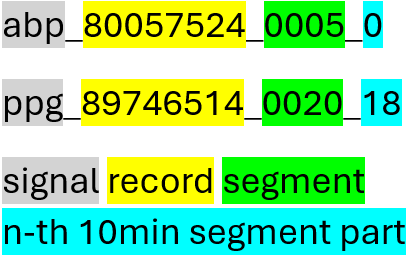
\includegraphics[width=0.3\textwidth]{images/methods/segments}
    \end{center}
    \vspace*{-7mm}
    \captionsetup{format=plain, justification=centering}
    \caption{\small Examples of extracted segment files}
    \label{fig:segments}
\end{wrapfigure}

As noted earlier, each subject in the database may encompass multiple studies, records, and segments.
To prevent disproportionate representation of individual patient data, a limit of 100 segments, each spanning 10 minutes, was imposed per subject.
This is specifically important for data retrieval from the MIMIC-III database, which is intended for training and testing purposes.
However, this restriction was not applied to data retrieval from the MIMIC-IV database, which is designated for validation purposes and aims to encompass all available 10-minute segments, thus simulating real-world data where over-representation is not a concern.

\begin{wrapfigure}{r}{0.35\textwidth}
    \vspace*{-5mm}
    \begin{center}
        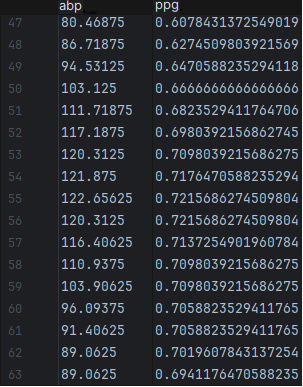
\includegraphics[width=0.3\textwidth]{images/methods/values}
    \end{center}
    \vspace*{-7mm}
    \captionsetup{format=plain, justification=centering}
    \caption{\small Example raw ABP and PPG values}
    \label{fig:values}
\end{wrapfigure}

Additionally, the primary objective was to achieve a dataset split ratio of 60/20/20 for training, testing, and validation, where 80\% of the data comprises the MIMIC-III dataset for training and testing (60/20), and the remaining 20\% consists of the MIMIC-IV dataset for validation purposes.
To facilitate this, an initial set of x segments was retrieved from the MIMIC-IV database, followed by obtaining four times the number of x segments from the MIMIC-III database.
However, it is important to acknowledge that the quantity of segments obtained from each database doesn't directly correspond to the number of features utilized in the ML phase, as signal processing (SP) tasks are performed in between.
Thus, the 60/20/20 split ratio for training, testing, and validation serves more as a guideline than an absolute target for the number of segments retrieved.
Details on achieving the actual proportions are provided in the subsequent section~\ref{subsec:sp_methods}.

% CODE in LATEX EXAMPLE
%\begin{lstlisting}[language=Python,label={lst:python}]
%    import wfdb
%
%    wfdb.get_record_list(db_name)
%    wfdb.rdrecord()
%    wfdb.rdheader()
%\end{lstlisting}

\subsection{Signal Processing}
\label{subsec:sp_methods}

\subsubsection{Filtering Aproaches}

butter + savgol optimal, because PPG shapes best (show pic)

\subsubsection{Beat Finding Algorithms}

3 beat findings algos from wfdb methods, 1 novel for reference

Beat grouping and synchronization

Mention that no manual selection was done, due to large size of samples

\subsubsection{Fiducial Point detection}

wfdb default algos

cave for dic notch

\subsubsection{Feature Extraction}

graphics for all 34 features

explain each significance

FFT formula

\subsection{Machine Learning}
\label{subsec:ml_methods}

LR, MLP, LSTM, GRU models tried

elaborate splitting approach

\begin{enumerate}

    \item Digital signal filtering using Savitzky-Golay and Butterworth Lowpass filters.

    \item Beat detection algorithms from MIMIC WFDB Tutorial used for primary estimation.
    Beat detection improved with manual implementation of SciPy library.

    \item Fiducial Point calculation based on the algorithm provided in the MIMIC WFDB Tutorial.

    \item Feature extraction with personally created code to extract time domain features, and NumPy library to extract frequency domain features (FFT). Median value calculation using NumPy library.

    \item Machine Learning Model creation using PyTorch and Scikit-Learn libraries.

\end{enumerate}
